\mychapter{Exames com QR+QM e/ou QT}\label{ch:examesQM_QT}

Este capítulo complementa o anterior, fornecendo detalhes sobre o processo de criação e correção de exames que envolvem tanto o Quadro de Respostas (QR) quanto os enunciados das questões de múltipla escolha (QMs), como exemplificado nos Capítulos \ref{ch:questoesClassicasMCTest} -- \nameref{ch:questoesClassicasMCTest} e  \ref{ch:questoesCodigoMCTest} -- \nameref{ch:questoesCodigoMCTest} para questões com código em Python.

Esse estilo de exame com QR+QM tem sido amplamente utilizado na Especialização em Tecnologia e Sistemas de Informação (TSI) da UFABC, como introduzido no Capítulo \ref{ch:introducao}, nos processos seletivos desde 2017. Anteriormente, desde 2012, já se utilizava o MCTest em versões anteriores, com QR+QM, porém em um formato de exame que empregava editores de texto como o Word ou o BROffice, com uma única folha frente e verso, para evitar a necessidade de grampear as folhas de milhares de candidatos nos processos seletivos. O avanço significativo no MCTest ocorreu na versão 4, quando passou a ser possível criar os exames utilizando o \LaTeX{}, o que permitiu também a inclusão de blocos de código Python para a elaboração de questões paramétricas, conforme apresentado no Capítulo \ref{ch:questoesCodigoMCTest} -- \nameref{ch:questoesCodigoMCTest}. A versão mais recente do MCTest, disponível na web, possibilitou o armazenamento das questões em um banco de dados, juntamente com toda uma estrutura para gerenciar um sistema acadêmico voltado exclusivamente para avaliações. Esses avanços têm sido objeto de diversas publicações e também motivaram a escrita deste livro, com o intuito de registrar as principais características de tudo o que foi desenvolvido e validado em avaliações dos mais diversos estilos.

Além das QMs, também é possível incluir questões dissertativas (QTs) nos exames, após a apresentação das QMs. Essa abordagem permite uma maior diversidade nos tipos de questões e uma avaliação mais abrangente das habilidades dos estudantes.

No Capítulo \ref{ch:exames} -- \nameref{ch:exames}, foi introduzido como criar exames contendo QR+QM, abordando detalhes sobre o formulário do exame. Agora, será colocada em prática a criação de exemplos de exames contendo QR+QM+QT, além de detalhar o processo de correção automática.

\section{Criando QMs e uma QT}\label{sec:questoesQM_QT}

Uma forma prática de criar questões não paramétricas no MCTest é utilizando um arquivo TXT com todas as questões, conforme introduzido na Seção \ref{sec:questaoNavegacao} -- \nameref{sec:questaoNavegacao}. Antes de prosseguir com a criação das questões, é necessário criar o tópico, por exemplo, \verb|DE-TIC| da disciplina, seguindo as instruções apresentadas na Seção \ref{sec:topicos} -- \nameref{sec:topicos}. 

A seguir, serão apresentadas sete questões que serão incluídas no MCTest. Serão duas questões para o nível de dificuldade fácil (\verb|QE|), ou dificuldade 1, duas questões para o nível de dificuldade médio (\verb|QM|), ou dificuldade 3, e três questões para o nível de dificuldade difícil (\verb|QH|), ou dificuldade 5. Para otimizar o processo de \textit{upload}, sugere-se agrupá-las em um único arquivo TXT.

\begin{myboxCode}{corCSV}{\textbf{Arquivo CSV, questões fáceis }}\vspace{3mm}
\hrule
{\footnotesize
\begin{verbatim}
QE::DE-TIC:: 
Qual é o componente principal de um computador que armazena dados e programas?
A: Memória RAM % alternativa correta - sempre a primeira
A: Placa-mãe
A: Processador
A: Teclado
A: Placa de vídeo

QE::DE-TIC:: 
Qual dos seguintes dispositivos é usado exclusivamente para entrada de dados em um computador?
A: Teclado 
A: Impressora
A: Caixa de som
A: Monitor
A: Placa de vídeo
\end{verbatim}
}
\end{myboxCode}

\begin{myboxCode}{corCSV}{\textbf{Arquivo CSV, questões de nível médio }}\vspace{3mm}
\hrule
{\footnotesize
\begin{verbatim}
QM::DE-TIC:: 
O que significa a sigla HTML?
A: HyperText Markup Language
A: High Technical Machine Language
A: Home Tool Management Language
A: Hyper Transfer Machine Learning
A: Hardware Technical Maintenance Language

QM::DE-TIC:: 
Qual das seguintes linguagens de programação é amplamente utilizada para o desenvolvimento de 
sites dinâmicos?
A: JavaScript
A: HTML
A: CSS
A: Python
A: C++
\end{verbatim}
}
\end{myboxCode}

\begin{myboxCode}{corCSV}{\textbf{Arquivo CSV, questões difíceis}}\vspace{3mm}
\hrule
{\footnotesize
\begin{verbatim}
QH::DE-TIC:: 
Qual das seguintes opções representa corretamente um endereço IP válido?
A: 127.0.0.1
A: 192.168.0.300
A: 10.0.0.256
A: 172.16.0.0
A: 256.256.256.256

QH::DE-TIC::
Qual dos seguintes protocolos de internet é utilizado para enviar e-mails?
A: SMTP
A: FTP
A: HTTP
A: DNS
A: SSH

QH::DE-TIC::
Qual é o resultado da soma dos números hexadecimais 7C e 54?
A: D0
A: F0
A: D4
A: D1
A: E0
\end{verbatim}
}
\end{myboxCode}

A questão apresentada no Código \ref{lst:questaoQT_exata} é um exemplo de QT que contém um valor exato como resposta correta, delimitado pelos marcadores \verb|%%{| e \verb|}%%|, conforme indicado na linha 5 do código. Neste caso, é utilizada a palavra ``exata'' como exemplo para ilustrar o funcionamento dessa abordagem. Na linha 7 do código, são desenhadas 10 linhas para que o estudante possa responder à questão. Na próxima seção, será explorada essa funcionalidade com mais detalhes.

\begin{listing}[!ht]
\begin{myboxCode}{corCodigo}{\textbf{Questão: }}\vspace{3mm}
\hrule
\begin{minted}[xleftmargin=20pt,linenos=true]{python}
Descreva brevemente a importância da tecnologia da informação (TI) na 
sociedade moderna e mencione pelo menos duas áreas onde a TI desempenha 
um papel fundamental.

%%{exata}%%

\drawLines{10}
\end{minted}
\end{myboxCode}
\caption{Exemplo de QT com resposta exata.}
\label{lst:questaoQT_exata}
\end{listing}



Ao criar o exame, selecione as sete QMs, escolhendo duas questões em cada nível de dificuldade, conforme ilustrado na Figura \ref{fig:cap08_figexameQR_QT}. Além disso, inclua uma QT como exemplo. Certifique-se de marcar a opção ``Respostas/Questões/Ambos=Ambos'' para incluir tanto o QR quanto as questões (QM e QT) no exame. Mais informações sobre essa configuração podem ser encontradas na Seção \ref{sec:exameDetalhes} -- \nameref{sec:exameDetalhes}.

\begin{figure}[!ht]
  \centering
  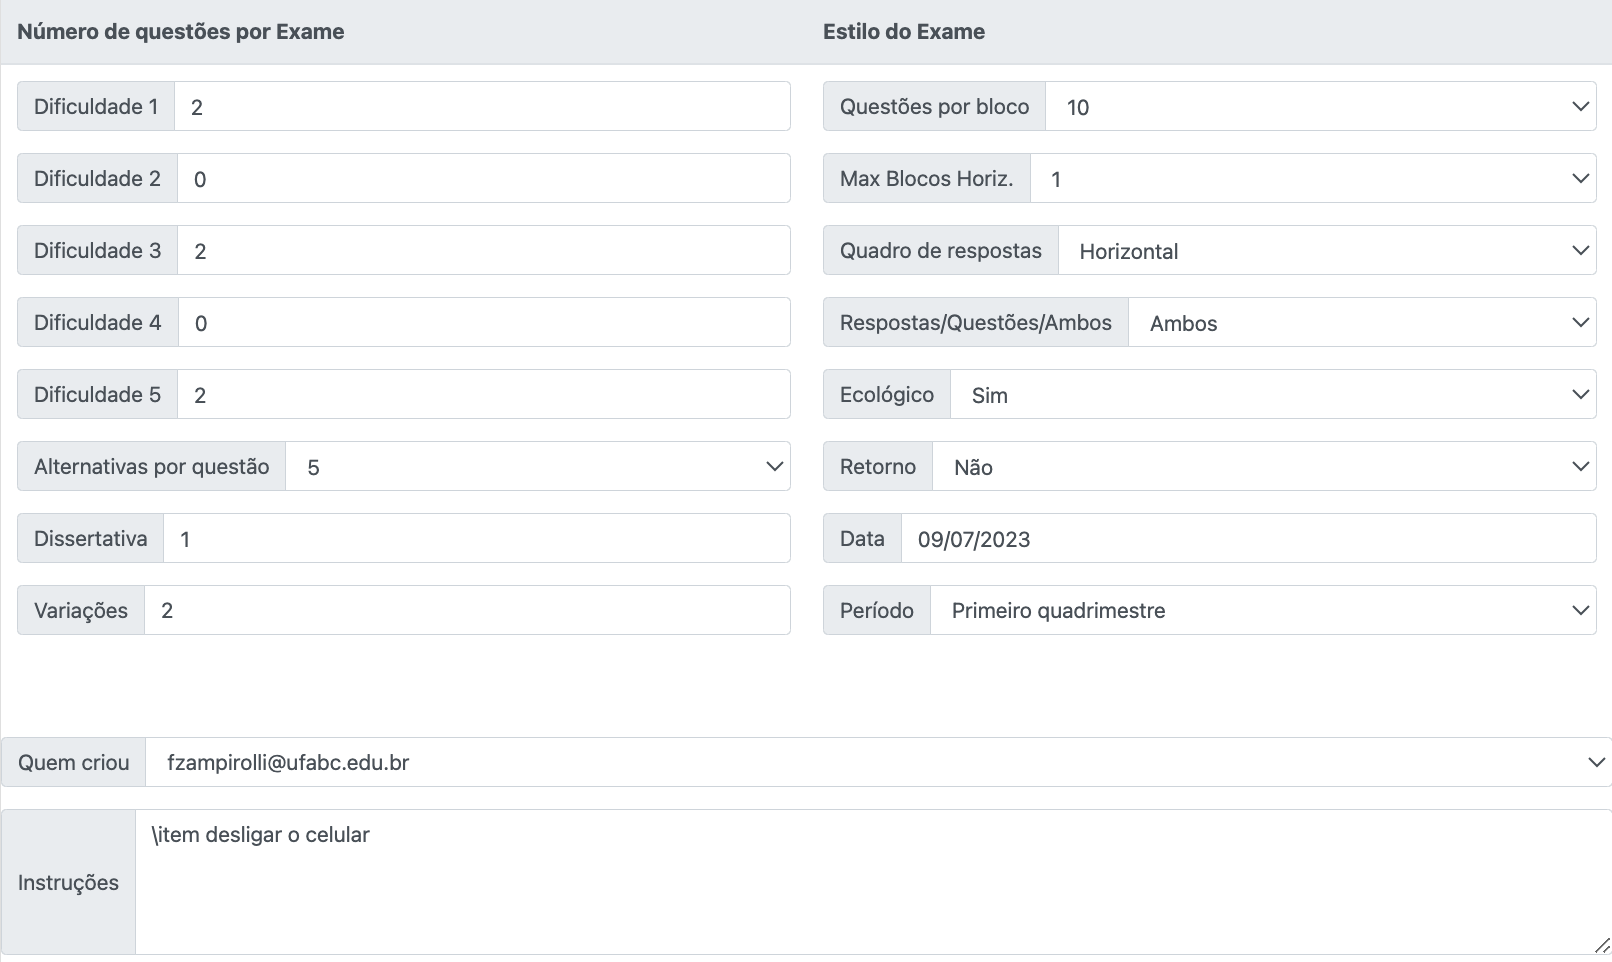
\includegraphics[width=0.9\textwidth]{cap08_figexameQR_QT.png}
   \caption{Recorte da tela de configuração do exame.}
\label{fig:cap08_figexameQR_QT}
\end{figure}

\section{Criando as variações}

Antes de criar o PDF do exame, é necessário criar as variações clicando no botão ``Criar-Variações'' (observe que ao lado deste botão há um ID inicialmente definido como 0, que será alterado quando o botão for pressionado). É importante detalhar mais essa opção, conforme ilustrado na Figura \ref{fig:cap08_figexameCriarVariacoes}.

Ao marcar a opção ``Json'', se a questão for de integração entre MCTest, Moodle e VPL, será enviado ao e-mail do professor um arquivo \verb|linker.json| contendo os casos de teste a serem incluídos na atividade VPL do Moodle. Se a opção ``Template'' for selecionada, será criado um arquivo CSV contendo o gabarito das QMs, bem como QTs com respostas curtas, para ser possível comparar as respostas exatas, caractere por caractere.

As opções ``Aiken'' e ``XML'' são utilizadas para gerar arquivos que podem ser importados para criar um banco de questões no Moodle. Por fim, ao selecionar a opção ``LaTeX+PDF'', o professor receberá um PDF contendo todas as variações do exame. No exemplo ilustrado na Figura \ref{fig:cap08_figexameQR_QT}, foram criadas apenas duas variações. Vale ressaltar que existem artigos validando cada método utilizado nesses botões, os quais serão detalhados na parte de experimentos deste livro.

\begin{figure}[!ht]
  \centering
  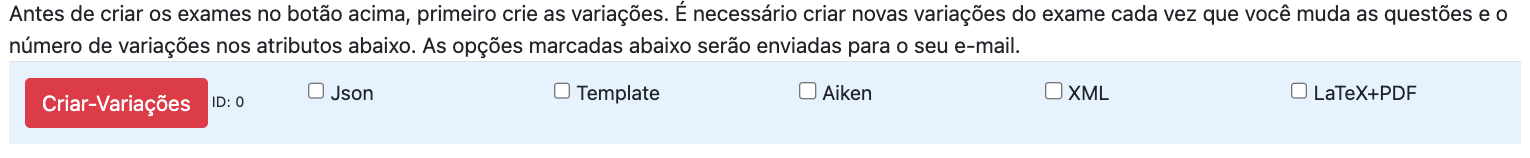
\includegraphics[width=0.9\textwidth]{cap08_figexameCriarVariacoes.png}
   \caption{Recorte da tela de configuração do exame, detalhando o botão ``Criar-Variações''.}
\label{fig:cap08_figexameCriarVariacoes}
\end{figure}

Assim, antes de criar o PDF do exame, marque a opção ``Template'' na Figura \ref{fig:cap08_figexameCriarVariacoes} para receber o gabarito e clique em ``Criar-Variações''. Nesse exemplo, uma nova aba será aberta no navegador exibindo a mensagem apresentada na Figura \ref{fig:cap08_figexameCriarVariacoesMsg}. 

\begin{figure}[!ht]
  \centering
  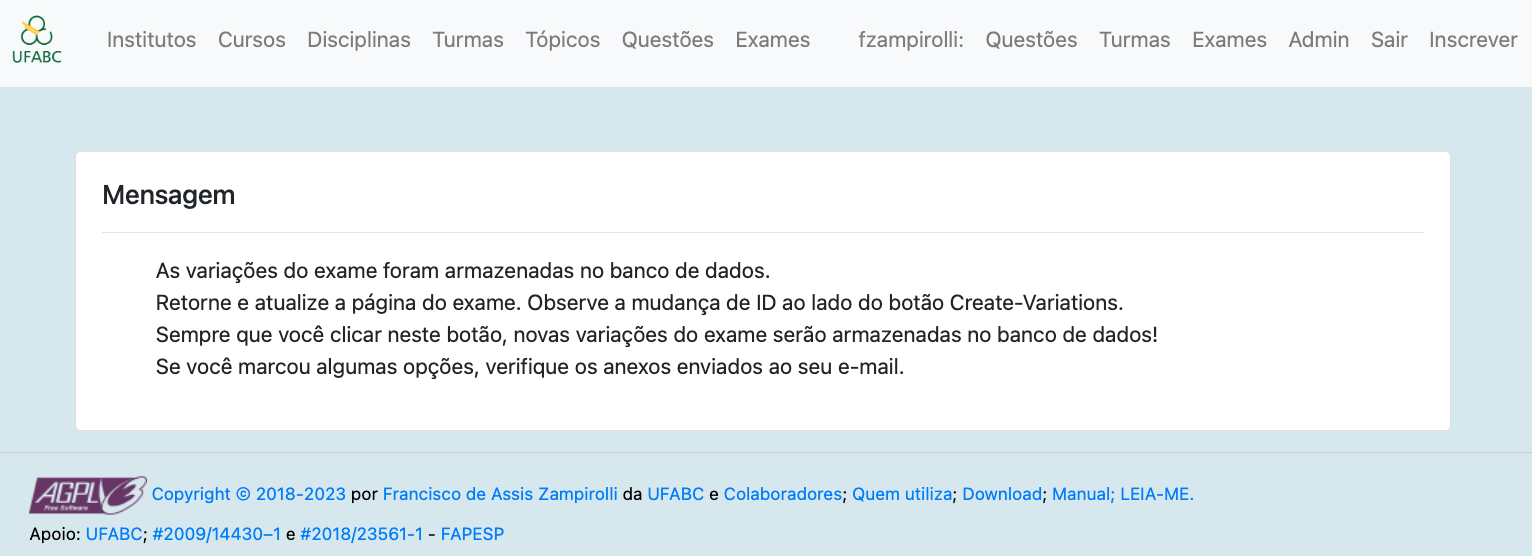
\includegraphics[width=0.9\textwidth]{cap08_figexameCriarVariacoesMsg.png}
   \caption{Mensagem após clicar no botão ``Criar-Variações''.}
\label{fig:cap08_figexameCriarVariacoesMsg}
\end{figure}


\section{Detalhando os gabaritos no arquivo CSV}\label{sec:QMgabarito}

Após clicar em ``Criar-Variações'', selecionando antes a opção ``Template'', o professor receberá um e-mail contendo o seguinte arquivo com os gabaritos, conforme ilustrado na Figura \ref{fig:cap08_figexameCriarVariacoesEmail}.

\begin{myboxCode}{corCSV}{\textbf{Arquivo CSV, com os gabaritos (as colunas são separadas por vírgula)}}\vspace{3mm}
\hrule
{\footnotesize
\begin{verbatim}
variation Q1 Q2 Q3 Q4 Q5 Q6    Q7     K1        K2        K3        K4        K5        K6
    0      A  B  C  A  A  A exata 245604231 245540123 245823041 245703214 245904132 246002413
    1      C  A  B  E  A  E exata 245612043 245503421 245830214 245741320 246104132 246032140
\end{verbatim}
}
\end{myboxCode}

\begin{figure}[!ht]
  \centering
  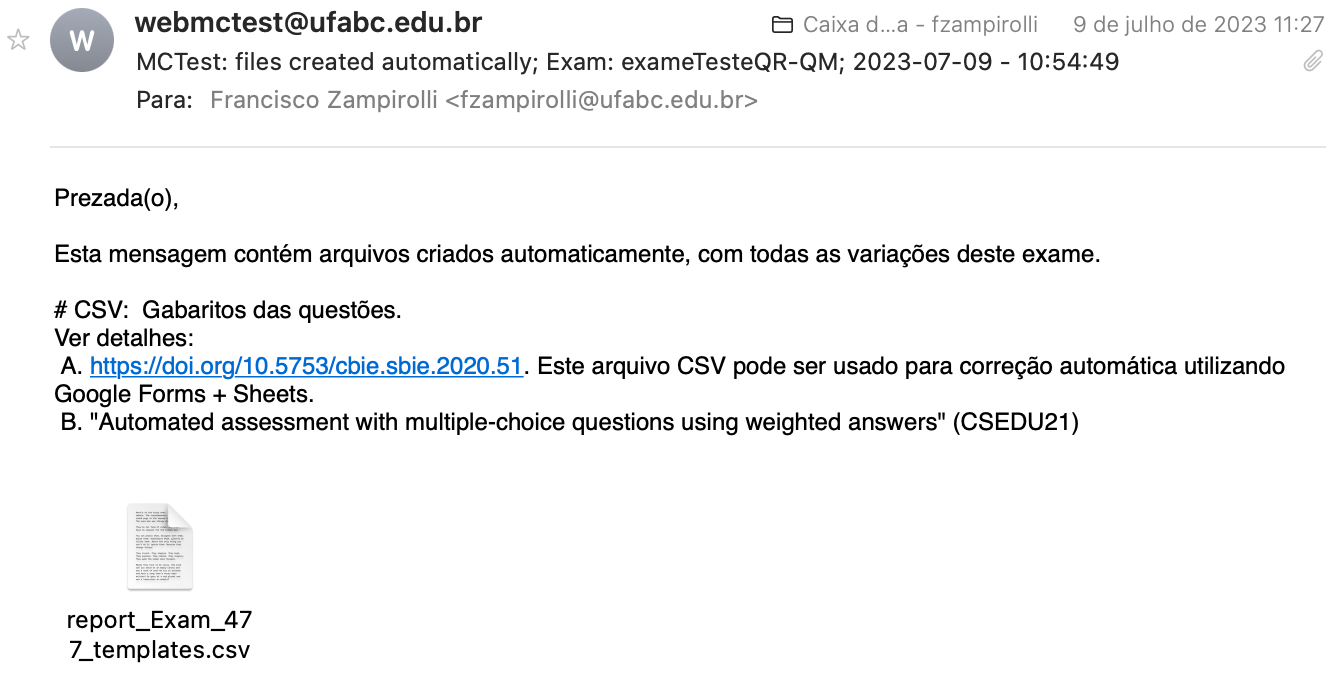
\includegraphics[width=0.9\textwidth]{cap08_figexameCriarVariacoesEmail.png}
   \caption{E-mail enviado ao professor após clicar no botão ``Criar-Variações''.}
\label{fig:cap08_figexameCriarVariacoesEmail}
\end{figure}


No arquivo em questão, a primeira coluna \verb|variation| apresenta a variação do exame. No exemplo mostrado na Figura \ref{fig:cap08_figexameQR_QT}, foram escolhidas apenas duas variações, identificadas como variação 0 e variação 1. Em seguida, são apresentadas as respostas corretas para cada uma das sete questões do exame, identificadas como \verb|Q1| até \verb|Q7|.

A questão \verb|Q7| é uma QT e foi definida em seu enunciado a sequência \verb|%%{exata}%%|, indicando para o MCTest que essa questão tem uma resposta exata contendo o texto ``exata''. É importante ressaltar que é possível incluir questões paramétricas, onde cada variação pode apresentar uma resposta correta diferente. Essa flexibilidade é discutida em detalhes no trabalho de \citeonline{2020:Zampirolli.Batista.ea}, que descreve a aplicação dessas técnicas na disciplina de Cálculo 1. Na parte de experimentos deste livro, essas abordagens serão apresentadas de forma mais detalhada, explorando suas aplicações e resultados.

Após as respostas corretas, são criadas novas colunas de \verb|K1| até \verb|K6| para detalhar o sorteio realizado em cada variação do exame para as QMs. Por exemplo, na variação 1 (segunda variação), a questão \verb|K1| tem o valor 245612043. Como são QMs com 5 alternativas, o valor 12043 indica a ordem das alternativas da questão 2456 (ID da questão no banco de dados). Sabendo que a alternativa correta sempre é a primeira (índice 0), pode-se concluir que a alternativa correta para essa questão é a letra C. Portanto, a alternativa A corresponde à segunda alternativa no banco de dados (índice 1), a alternativa B corresponde à terceira (índice 2), a alternativa C corresponde à primeira correta (índice 0), a alternativa D corresponde à quinta (índice 4) e a alternativa E corresponde à quarta (índice 3), resultando na sequência 12043. 

Ao analisar o sorteio das questões em ambas as variações, foram selecionadas sete QMs. No entanto, para cada exame, apenas seis questões serão sorteadas, conforme a configuração previamente definida. No arquivo CSV, é possível observar que apenas a questão \verb|Q5| apresentou variações diferentes das demais questões (consulte a coluna \verb|K5|, com questões de ID 2459 e 2461).

Uma estrutura de atribuição de pesos diferentes para cada alternativa marcada é detalhada no trabalho de  \citeonline{2020:Zampirolli.Batista.ea}, onde são apresentadas abordagens para avaliar o desempenho dos estudantes considerando a relevância das respostas em QMs.

\begin{mybox}{corCopia}{\textbf{Atenção:\\\vspace{-3mm}\hrule\vspace{3mm}}}
É extremamente importante verificar se o gabarito gerado corresponde ao PDF que será distribuído aos estudantes.
\begin{enumerate}
\item O ID da variação será alterado toda vez que o botão ``Criar-Variações'' for acionado;
\item Esse número de ID também será impresso no PDF gerado, abaixo do cabeçalho do exame, em vermelho. Por exemplo, {\color{red} \verb|#E477#V60970 -- 2023-07-09 -- 14:58:34|}. No exemplo mencionado, o exame possui o ID 477 e a variação é 60970;
\item No momento em que o botão ``Criar-Variações'' é acionado, uma ``fotografia'' das questões selecionadas no exame é armazenada no banco de dados para cada variação. Essa ``fotografia'' representa o estado atual das questões e é independente de eventuais alterações realizadas posteriormente pelo coordenador da disciplina ou professor que criou alguma destas questões. Esse recurso de segurança garante que as variações do exame permaneçam consistentes, mesmo que haja modificações nas questões originais.
\end{enumerate}
\end{mybox}


\section{Criando o PDF do exame com QR+QM+QT}\label{sec:exameQM_QT_criarPDF}

Após a criação das variações, a próxima etapa do processo de criação do exame consiste em gerar o PDF contendo os QRs, as QMs e QTs, caso estejam presentes no exame. Essa etapa é realizada ao clicar no botão ``Criar-PDF'' no painel de configuração do exame.

Ao gerar o PDF, todas as variações do exame serão incluídas, garantindo a diversificação das questões e respostas. Os QRs serão apresentados para os estudantes poderem preencher suas respostas, e as QMs e QTs serão apresentadas conforme a configuração do exame. A ordem das questões impressas no PDF gerado segue a ordem de dificuldade de 1 a 5 para as QMs. Em seguida, as QTs serão apresentadas na mesma ordem.

É de extrema importância revisar o PDF gerado para garantir a correta formatação das questões, respostas e demais elementos antes de disponibilizá-lo aos estudantes.
%
Além disso, é válido ressaltar que será criado um PDF para cada turma selecionada no exame, conforme detalhado na Seção \ref{sec:exameTurmas} -- \nameref{sec:exameTurmas}. No contexto do exame criado nas seções anteriores, foi gerado o PDF ilustrado na Figura \ref{fig:cap08_figexameQR_QM_QT_PDF}. 

\begin{figure}[!ht]
  \centering
  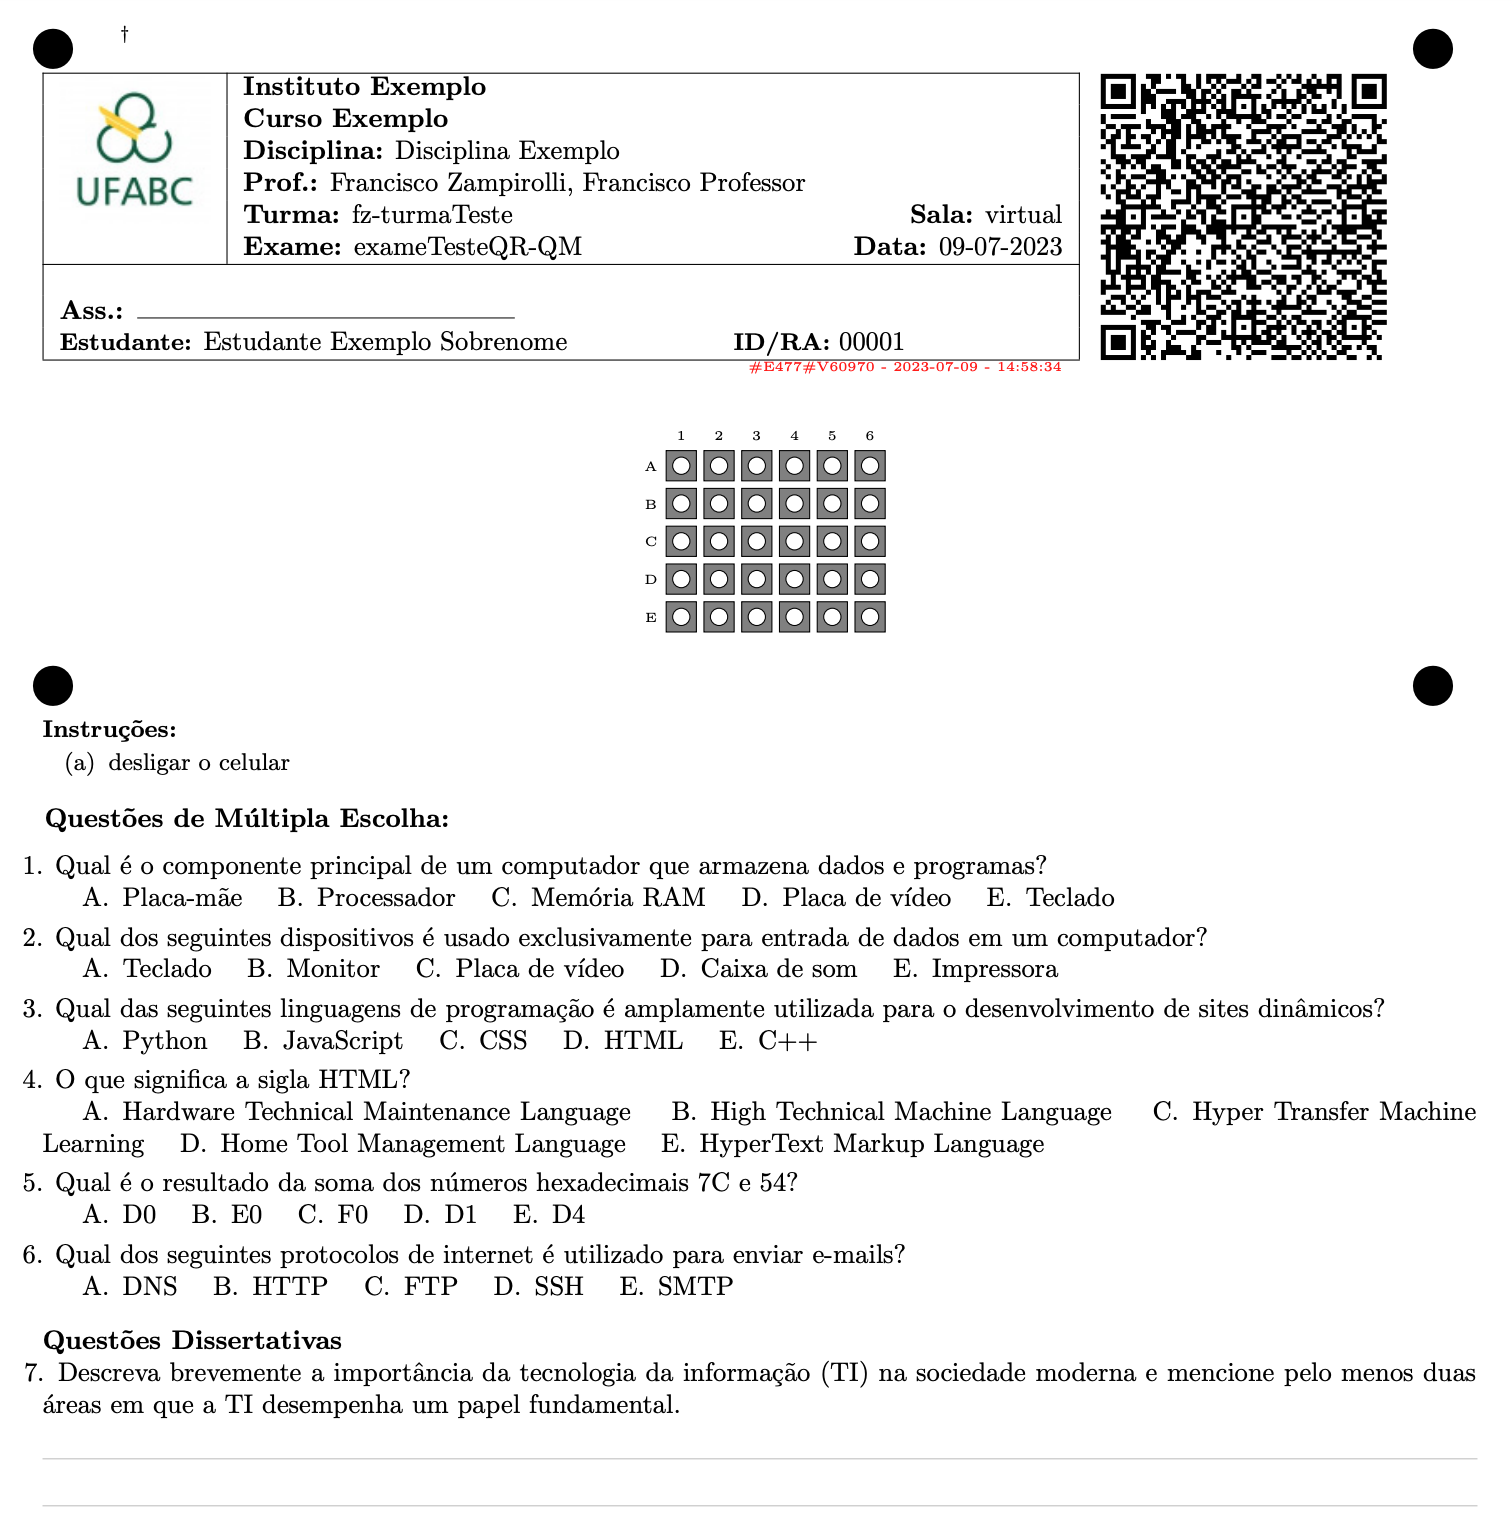
\includegraphics[width=0.9\textwidth]{cap08_figexameQR_QM_QT_PDF.png}
   \caption{Recorte do PDF do exame gerado após a ação do botão ``Criar-PDF''.}
\label{fig:cap08_figexameQR_QM_QT_PDF}
\end{figure}

Após a geração do PDF do exame, será enviado por e-mail ao professor o arquivo \LaTeX{} correspondente a cada turma selecionada. Esse arquivo pode ser útil caso o professor deseje realizar alterações manuais no exame, embora seja importante ressaltar que o QRcode é específico de cada estudante, para garantir a correção automática. No exemplo fornecido, o arquivo gerado é o \verb|_e477_class_670_varID_60970.tex|. 

Além do arquivo \LaTeX{}, o e-mail também conterá um arquivo CSV anexado, que apresenta as variações sorteadas para cada estudante. No exemplo mencionado, o arquivo é denominado \verb|report_Exam_477_varID_60970_students_variations.csv|. Caso haja mais turmas selecionadas para o exame, todos os estudantes de todas as turmas serão listados em um único arquivo CSV, que corresponde ao exame com o ID 477.

% melhorar escrita formal e científica, mantendo a formatação LaTex: 
Ao observar a Figura \ref{fig:cap08_figexameCriarPDF_Email}, é possível verificar um trecho do e-mail encaminhado ao professor após acionar o botão ``Criar-PDF'' contendo os três arquivos a seguir:

\begin{myboxCode}{corCSV}{\textbf{Arquivos anexados ao e-mail enviado ao professor}}\vspace{3mm}
\hrule
\begin{verbatim}
_e477_varID_60970_class_670.pdf
_e477_varID_60970_class_670.tex
_e477_varID_60970_class_670_students_variations.csv
_e477_varID_60970_class_670_variations.csv
\end{verbatim}
\end{myboxCode}
 
\begin{figure}[!ht]
  \centering
  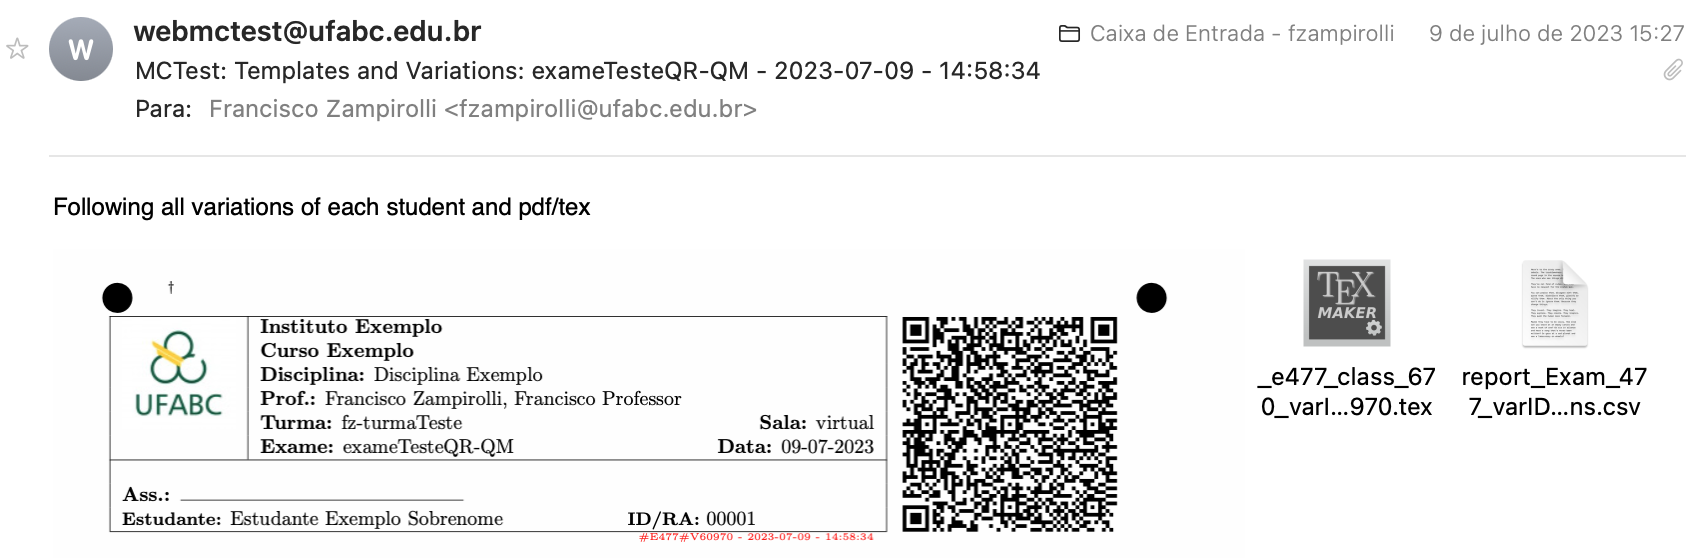
\includegraphics[width=0.9\textwidth]{cap08_figexameCriarPDF_Email.png}
   \caption{E-mail enviado ao professor após clicar no botão ``Criar-PDF''.}
\label{fig:cap08_figexameCriarPDF_Email}
\end{figure}


\begin{myboxCode}{corCSV}{\textbf{Arquivo \texttt{\_e477\_varID\_60970\_students\_variations.csv}, com as variações de cada estudante}}\vspace{3mm}
\hrule
\begin{verbatim}
Name                          Variation
Estudante Exemplo Sobrenome      1
\end{verbatim}
\end{myboxCode}

\begin{myboxCode}{corCSV}{\textbf{Arquivo \texttt{\_e477\_varID\_60970\_variations.csv}, com as variações de cada estudante, com turma e soma das notas de exames anteriores}}\vspace{3mm}
\hrule
\begin{verbatim}
Room           ID     Name                 Variation SumLatestGrades
fz-turmaTeste 00001 Estudante Exemplo Sobrenome 1          0
\end{verbatim}
\end{myboxCode}

\begin{mybox}{corCopia}{\textbf{Atenção:\\\vspace{-3mm}\hrule\vspace{3mm}}}
Foi adotado o seguinte critério de sorteio de variações para os estudantes:
\begin{enumerate}
\item Se o número de variações definido for menor que o número de estudantes em cada turma, será sorteada uma variação para os estudantes  baseado no \textit{hash} gerado a partir do nome e sobrenome do estudante. Dessa forma, ao clicar em ``Criar-PDF'', será atribuída a mesma variação para cada estudante;
\item Caso contrário, ou seja, se o número de variações definido no exame for maior ou igual que o número de estudantes da turma, será sorteada uma variação diferente para cada estudante a cada vez que o botão ``Criar-PDF'' for acionado.
\end{enumerate}
\end{mybox}

\section{Corrigindo exames com QR+QM}


Ao corrigir exames que contêm QR e QMs utilizando o MCTest, o processo é mais simples em comparação com a correção de exames apenas com QR, conforme detalhado na Seção \ref{sec:examesCorrigirQR} -- \nameref{sec:examesCorrigirQR}.

O gabarito de cada exame é armazenado no servidor do MCTest. Ele é identificado através da decodificação do QRcode, sendo criptografado e compactado, como ilustrado na Figura \ref{fig:cap08_figexameQR_QM_QT_PDF}.

É possível verificar as respostas correspondentes ao gabarito apresentado no CSV na Seção \ref{sec:QMgabarito} -- \nameref{sec:QMgabarito}, considerando a variação 1, conforme apresentado no CSV da seção anterior. Portanto, as respostas para as questões \verb|Q1| até \verb|Q7| são, respectivamente: \verb|C, A, B, E, A, E, exata|.

Imprimindo o PDF apresentado na Figura \ref{fig:cap08_figexameQR_QM_QT_PDF}, selecionando a opção ``Retorno=Sim'' e salvando o exame, preenchendo as questões, digitalizando e enviando para o botão ``Upload-PDF'',  o estudante receberá o \textit{feedback} apresentado na Figura \ref{fig:cap08_figexameQR_QM_QT_PDFScan} por e-mail.


\begin{figure}[!ht]
  \centering
  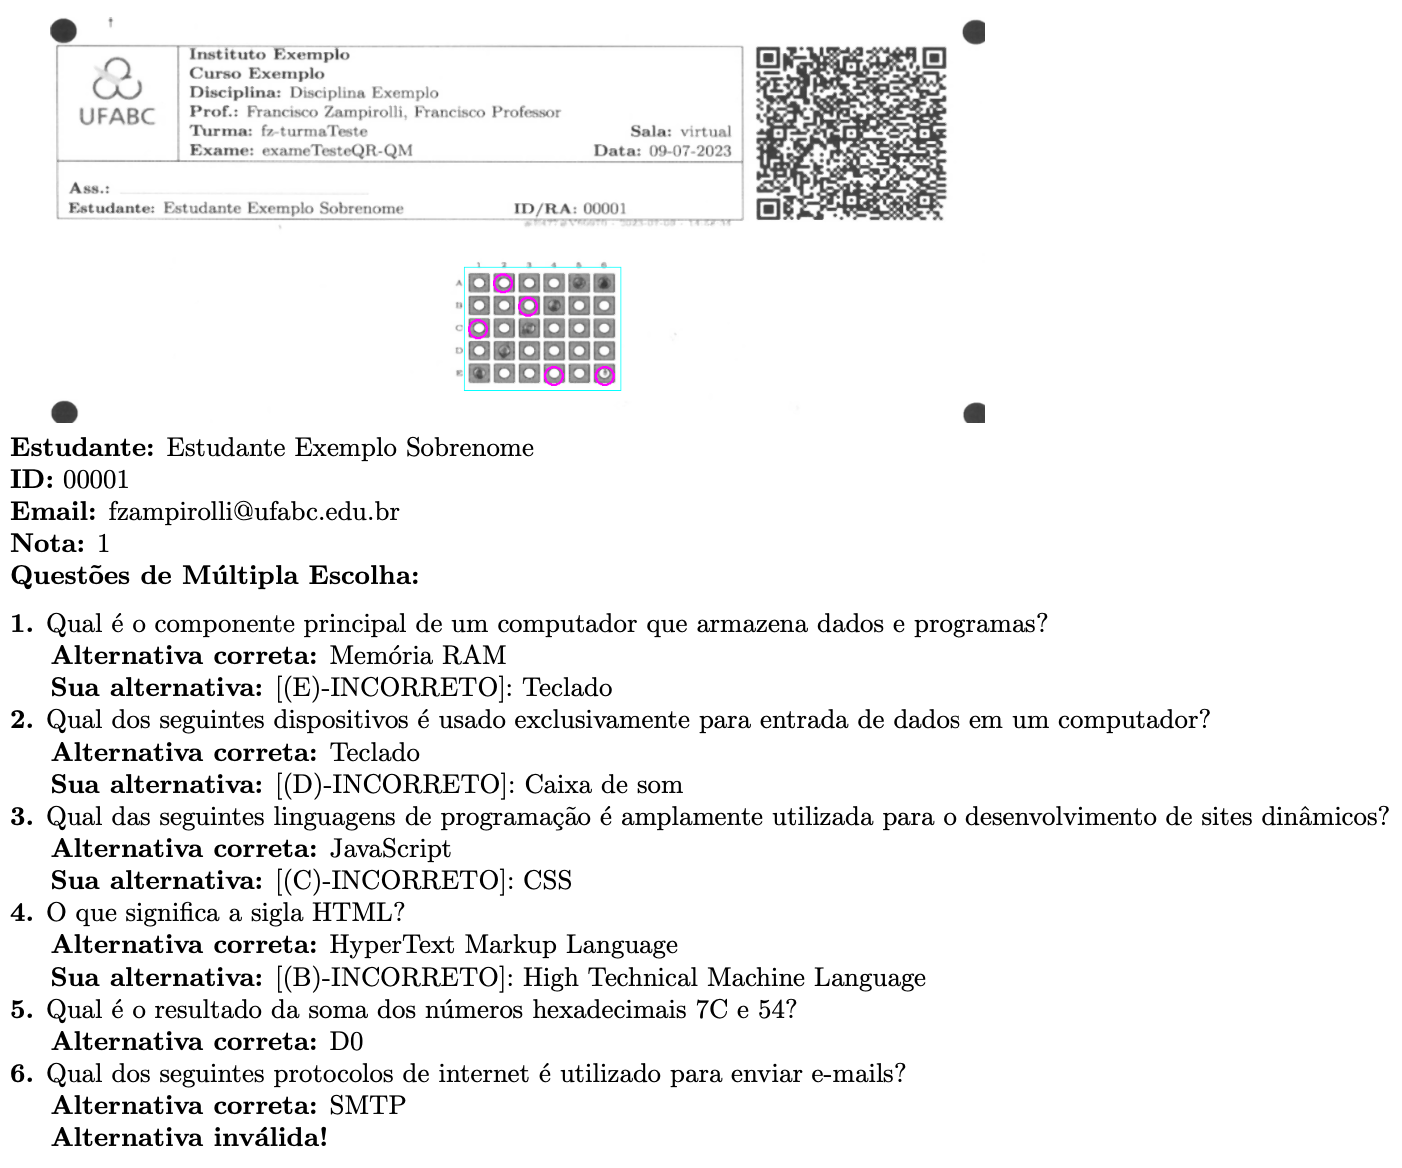
\includegraphics[width=0.9\textwidth]{cap08_figexameQR_QM_QT_PDFScan.png}
   \caption{Recorte do e-mail com parte do PDF do exame enviado como \textit{feedaback} ao estudante, após a ação do botão ``Upload-PDF''.}
\label{fig:cap08_figexameQR_QM_QT_PDFScan} 
\end{figure}

Além disso, o professor receberá as correções realizadas em um arquivo ZIP, conforme detalhado na Seção \ref{sec:examesCorrigirQR}, que conterá os seguintes arquivos:
 
\begin{myboxCode}{corCSV}{\textbf{Arquivos gerados ao solicitar a correção do exame no botão ``Upload-PDF''}}\vspace{3mm}
\hrule
\begin{verbatim}
studentEmail_e477.zip
_e477_fzampirolli@ufabc.edu.br_ScanFileQR_QM_RETURN__.csv
_e477_fzampirolli@ufabc.edu.br_ScanFileQR_QM_RETURN_irt.csv
_e477_fzampirolli@ufabc.edu.br_ScanFileQR_QM_RETURN_p001_s1_q006.png
_e477_fzampirolli@ufabc.edu.br_ScanFileQR_QM_RETURN_statistics.csv
\end{verbatim}
\end{myboxCode}

O arquivo \verb|studentEmail_e477.zip| contém todos os arquivos PDF enviados aos estudantes, caso tenham escolhido ``Retorno=SIM'' no formulário do exame. Um exemplo é apresentado na Figura \ref{fig:cap08_figexameQR_QM_QT_PDFScan}, exibindo também as questões, as respostas do estudante e a alternativa correta. Esses enunciados são incluídos no PDF quando a caixa abaixo do botão ``Upload-PDF'' é marcada; caso contrário, apenas a imagem, as informações do estudante e sua nota são enviadas. 

\begin{mybox}{corEdicao2}{\textbf{Destaque:\\\vspace{-3mm}\hrule\vspace{3mm}}}
  Um destaque incluído na versão mais recente do MCTest é apresentar as questões e as alternativas armazenadas nas variações salvas no banco de dados. Ou seja, quando há questões paramétricas, é exibida a ``fotografia'' da questão criada no momento em que o botão ``Criar-Variações'' foi pressionado. Já o \textit{feedback} é apresentado obtendo o atributo da própria questão, que não pode ser parametrizado e pode ser alterado a qualquer momento, sendo incluído no PDF a ser enviado ao estudante. Para isso, foi necessário incluir no QRCode informações da chave da variação do exame sorteada para cada estudante.
\end{mybox}

Conforme explicado na Seção \ref{sec:CSVcorrecoesQR} -- \nameref{sec:CSVcorrecoesQR}, o primeiro arquivo CSV, \verb|*_.csv|, apresenta o seguinte conteúdo:

% \tiny < \scriptsize < \footnotesize < \small 

\begin{myboxCode}{corCSV}{\textbf{Conteúdo do arquivo \texttt{*\_.csv} gerado (as colunas são separadas por vírgula)}}\vspace{3mm}
\hrule
{\scriptsize
\begin{verbatim}
Pag ID Resp Quest Inv Grad Q1  Q2  Q3  Q4 Q5 Q6     K1        K2        K3        K4        K5        K6
1  001    5     6   1   1 E/C D/A C/B B/E A 2/E 245612043 245503421 245830214 245741320 246104132 246032140
\end{verbatim}
}
\end{myboxCode}


% melhorar escrita formal e científica, mantendo a formatação LaTex: 

No arquivo em questão, é possível observar nas colunas \verb|Q1| até \verb|Q6| a notação apresentada na Seção \ref{sec:CSVcorrecoesQR}, agora com a adição de \verb|resposta marcada/resposta correta|. Por exemplo, na questão \verb|Q1| tem a notação \verb|E/C|, indicando que a alternativa marcada pelo estudante foi a \verb|E|, enquanto a resposta correta é a \verb|C|. Também é possível notar a presença de uma questão inválida na coluna \verb|Inv|, referente à questão \verb|Q6|, que apresenta o conteúdo \verb|2/E|. Isso indica que duas alternativas foram marcadas, sendo que na Figura \ref{fig:cap08_figexameQR_QM_QT_PDFScan} é possível observar que a alternativa \verb|A| foi marcada, mas também foi realizada uma pequena marcação na alternativa \verb|E|, invalidando a questão. Neste exemplo, a única marcação correta é na questão \verb|Q5|.

A Figura \ref{fig:cap08_figexameQR_QM_QT_PDFScan} apresenta um relatório com os dados do estudante, a nota obtida e os enunciados das questões, incluindo as marcações realizadas e a alternativa correta de cada questão. As colunas \verb|K1| até \verb|K6| foram previamente explicadas na Seção \ref{sec:QMgabarito} -- \nameref{sec:QMgabarito}.

% NOVO
\section{Exames adaptativos}\label{sec:testeAdaptativo}

Abaixo do botão ``Criar-PDF'' na tela de exame, conforme ilustrado na Figura \ref{fig:cap06_figExameAtualiza1}, encontram-se duas barras de rolagem. A primeira permite definir o tamanho da fonte do arquivo PDF gerado com o exame. A segunda barra de rolagem possibilita definir o número de exames anteriores realizados por cada estudante a ser considerado. Por exemplo, se o valor selecionado for 1, será considerada apenas a nota do último exame para definir qual variação deste será destinada aos estudantes.

Para que este método de exame adaptativo funcione adequadamente, é necessário definir a taxonomia de Bloom para cada questão, nos 6 possíveis níveis: lembrar, compreender, aplicar, analisar, avaliar e criar. Cada um desses níveis recebe um valor de 1 a 6, respectivamente. Quando, para cada nível de dificuldade, são escolhidas várias questões com taxonomias distintas, cada variação do exame poderá apresentar pesos diferentes considerando essas taxonomias. Por exemplo, se um exame definir 5 questões com dificuldade 1, porém houver 10 questões marcadas para esse mesmo nível 1, além disso, foi decidida a criação de 20 variações de exames, teremos então variações com somatórios distintos dos pesos dos níveis dessa taxonomia.

Para ilustrar esse processo, foi criado um exame com 3 QM e 1 QT, todas com dificuldade 1. Além disso, foram selecionadas 6 QM para serem sorteadas, com apenas 3 delas sendo escolhidas com base no desempenho do estudante em exames recentes. Na barra de rolagem, foi escolhido o número 6 para o exame adaptativo, ou seja, serão somadas as 6 últimas notas dos exames realizados pelo estudante. Foram solicitadas a criação de 20 variações de exames após clicar no botão ``Criar-Variações''. Também foram selecionadas duas turmas. Após clicar no botão ``Criar-PDF'', os arquivos foram enviados para o email do professor, além de um \textit{download} de um arquivo compactado contendo os seguintes arquivos.

\begin{myboxCode}{corCSV}{\textbf{Arquivos gerados ao solicitar criar PDF com o botão``Criar-PDF''}}\vspace{3mm}
\hrule
\begin{verbatim}
_e482_varID_61011_adaptive_test.csv
_e482_varID_61011_adaptive_test_variations_by_bloom.csv
_e482_varID_61011_class_669.pdf
_e482_varID_61011_class_669.tex
_e482_varID_61011_class_670.pdf
_e482_varID_61011_class_670.tex
_e482_varID_61011_students_variations.csv
_e482_varID_61011_variations.csv
\end{verbatim}
\end{myboxCode}

O primeiro arquivo \verb|_e482_varID_61011_adaptive_test.csv| possui na primeira coluna as 20 variações do exame, na segunda coluna a chave das variações no BD e na terceira coluna a soma dos níveis da taxonomia de Bloom para as questões sorteadas para cada variação, em ordem crescente. Observam-se as questões com variações 7 e 13 com o mesmo nível de dificuldade 7. Além disso, apenas a variação 9 tem dificuldade 15.

\begin{myboxCode}{corCSV}{\textbf{Arquivo \texttt{\_e482\_varID\_61011\_adaptive\_test.csv}}}\vspace{3mm}
\hrule
\begin{verbatim}
Variation  VariationID  SumBloomQuestions
 7            61017        7
13            61023        7
 6            61016        8
12            61022        9
14            61024        9
15            61025        9
17            61027        9
 3            61013       10
 4            61014       10
20            61030       10
16            61026       11
18            61028       11
 2            61012       12
 8            61018       12
11            61021       12
 1            61011       13
10            61020       13
19            61029       13
 5            61015       14
 9            61019       15
\end{verbatim}
\end{myboxCode}


\begin{myboxCode}{corCSV}{\textbf{Arquivo \texttt{\_e482\_varID\_61011\_adaptive\_test.csv}}}\vspace{3mm}
\hrule
\begin{verbatim}
RoomID RoomCode      NomeAluno                             EmailAluno               
670    fz-turmaTeste Estudante Exemplo Sobrenome           fzampirolli@ufabc.edu.br 
669    Turma Exemplo João da Silva                         joao@aluno.ufabc.edu.br  
669    Turma Exemplo Maria da Silva Andrade de S Gonçalves maria@aluno.ufabc.edu.br 
\end{verbatim}
\end{myboxCode}

\begin{myboxCode}{corCSV}{\textbf{Continuação do arquivo \texttt{\_e482\_varID\_61011\_adaptive\_test.csv}}}\vspace{3mm}
  \hrule
  \begin{verbatim}
IDExame1 DataExame1 GradeExame1  IDExame2 DataExame2  GradeExame2 
476      2023-07-06 18.0         477      2023-07-09  1.0         
475      2023-04-17              482      2023-11-19  0.0  
475      2023-04-17              482      2023-11-19  0.0   
\end{verbatim}
\end{myboxCode}


\begin{myboxCode}{corCSV}{\textbf{Continuação do arquivo \texttt{\_e482\_varID\_61011\_adaptive\_test.csv}}}\vspace{3mm}
\hrule
\begin{verbatim}
DExame3 DataExame3  SumLatestGrades
478.0    2023-07-11  19.0
  
 
\end{verbatim}
\end{myboxCode}

O último valor de cada linha representa o somatório das últimas 6 avaliações do estudante. As avaliações de 4 a 6 não foram apresentadas, pois não tiveram notas associadas. O arquivo \verb|_e482_varID_61011_variations.csv| a seguir resume esses dados, com a variação sorteada para cada estudante. Observa-se que as duas variações (7 e 13) com a menor soma pela taxonomia de Bloom (7) foram sorteadas para os alunos da turma \verb|Turma Exemplo|.

\begin{myboxCode}{corCSV}{\textbf{Arquivo \texttt{\_e482\_varID\_61011\_variations.csv}}}\vspace{3mm}
\hrule
\begin{verbatim}
Room          ID  Name                               Variation  SumLatestGrades
fz-turmaTeste   1 Estudante Exemplo Sobrenome             9            19.0
Turma Exemplo 123 João da Silva                           7            0.0
Turma Exemplo 987 Maria da Silva Andrade de S Gonçalves  13            0.0
\end{verbatim}
\end{myboxCode}


Uma parte crucial desse processo adaptativo é a seleção apropriada das questões, classificadas com base na taxonomia de Bloom. É essencial garantir que as questões sejam bem definidas e alinhadas aos objetivos de aprendizagem. Além disso, esse método adaptativo deve motivar os estudantes a permanecerem engajados na disciplina, evitando a imposição de exames excessivamente difíceis como forma de penalização ou demasiadamente fáceis, o que resultaria em atribuição injusta de conceitos.


% melhorar escrita formal e científica, mantendo a formatação LaTex: 

\section{Recomendações para realização tranquila de exames presenciais}\label{sec:recomendacoesCap8}

Com base na experiência de inúmeros exames aplicados e corrigidos, é possível destacar algumas recomendações essenciais para garantir a realização tranquila do processo e permitir o melhor desempenho de todos os envolvidos:

\begin{enumerate}
    \item Revisar cuidadosamente todas as questões, a fim de evitar erros ou ambiguidades que comprometam a aplicação ou correção. Questões mal elaboradas podem prejudicar a validade de todo o exame;
    \item Após selecionar as questões e configurar o estilo, crie as variações de exame marcando a caixa ``Template'' ao lado do botão ``Criar-Variações''. Isso assegura que o sistema gere os gabaritos corretos e possibilite a correção automática por meio do QRCode (se houver algum erro na leitura do QRCode durante a correção automática, o gabarito enviado por e-mail deverá ser usado -- certifique-se de guardar o arquivo CSV com cuidado);
    \item Cada vez que você clicar em ``Criar-Variações'', o ID será alterado, gerando novas variações com gabaritos diferentes no banco de dados. Para aplicar o exame, verifique se o ID ao lado deste botão corresponde ao ID em vermelho no PDF do exame (não se esqueça de atualizar a página para atualizar o ID). Isso é fundamental para garantir a correção automática, pois o ID gerado deve sempre coincidir com o do exame aplicado;
    \item É viável empregar as variações existentes no banco de dados em múltiplas turmas, com a simples modificação da turma no exame, seguida dos botões ``Salvar'' e ``Criar-PDF'';
    \item Deixar ``Retorno'' como ``Não'' ao criar os exames, caso contrário elas serão enviadas aos estudantes por e-mail antes da aplicação;
    \item Imprima um único exemplar do exame antes de produzir toda a tiragem, a fim de validar. Preencha o exame, digitalize e solicite a correção automática enviando o PDF e selecionando o botão ``Upload-PDF''. Isso permite verificar se o sistema gerou o exame corretamente e realizou a correção automática adequadamente. Além disso, verifique se todos os exames ocupam apenas uma página frente e verso, evitando a necessidade de grampear folhas. Se todos os PDFs gerados estiverem corretos, solicite a impressão no modo frente e verso, utilizando uma impressora com bom toner. Por fim, verifique se a impressão foi realizada com sucesso, garantindo que os quatro discos pretos que delimitam o QR estão intactos e sem cortes na folha;
    \item Organizar os exames em ordem alfabética sobre as filas de carteiras da sala, de modo que os estudantes não tenham dúvidas sobre qual é a deles. Isso garante que todos tenham acesso aos seus exames de forma rápida e organizada. Esse processo geralmente leva cerca de 10 minutos para 100 exames;
    \item Instrua os estudantes a não utilizar fluidos de correção (conhecidos como ``branquinho'') ou fazer rascunhos nos espaços designados pelos quatro discos pretos, a fim de evitar a interferência na correção automática dos gabaritos;
    \item Digitalizar somente a frente dos exames em um único arquivo PDF por turma para permitir a correção em larga escala de maneira ágil e livre de erros. Evite o uso de impressoras que possam ``engolir'' as folhas;
    \item Se ocorrer erro na decodificação do QRCode, é possível digitalizar apenas os exames com erro, utilizando diferentes configurações de digitalização da impressora. Outra alternativa é a correção manual, usando o gabarito enviado por e-mail. Certifique-se de verificar qual é a variação do exame do estudante recebido por e-mail ao clicar em ``Criar-PDF'' e o gabarito da variação recebida também por e-mail ao clicar em ``Criar Variação'';
    \item Envie os resultados aos estudantes somente após validar as correções para assegurar que tudo ocorreu conforme o esperado e não há erros. Se desejar enviar um gabarito aos estudantes apenas com QR, sem as questões, marque ``Retorno'' como ``SIM'' e não selecione a caixa abaixo do botão ``Upload-PDF''. Em seguida, escolha o arquivo e clique no botão para realizar a correção automática e enviar os \textit{feedbacks} aos estudantes por e-mail.
\end{enumerate}

Seguir essas recomendações é crucial para a realização de exames presenciais tranquilamente. É essencial revisar as questões, criar variações e verificar os IDs tanto na página do exame quanto no PDF. Garantir a impressão correta do PDF, sem cortes no QR, é importante. Além disso, realizar a validação das correções antes de enviar os resultados assegura a qualidade e precisão do processo. Ao seguir essas recomendações, é possível promover a eficiência da correção automatizada.

\section{Considerações finais}

Este capítulo abordou a criação e correção de exames que envolvem tanto o QR quanto as QMs, além das QTs. Essa combinação de questões permite uma avaliação abrangente das habilidades dos estudantes e tem sido amplamente utilizada na Especialização em Tecnologia e Sistemas de Informação (TSI) da UFABC, como mencionado no Capítulo \ref{ch:introducao}.

No processo de criação dos exames, é necessário criar as QMs e QTs, seguindo as instruções fornecidas neste capítulo, bem como nos Capítulos \ref{ch:questoesClassicasMCTest} -- \nameref{ch:questoesClassicasMCTest} e \ref{ch:questoesCodigoMCTest} -- \nameref{ch:questoesCodigoMCTest}. A utilização de arquivos TXT para criar as questões não paramétricas é uma abordagem prática e eficiente para inseri-las no MCTest. Além disso, é fundamental criar as variações do exame por meio do botão ``Criar-Variações''. Essa etapa garante a diversificação das questões e respostas disponibilizadas aos estudantes.

Após a criação das variações, é possível gerar o PDF do exame, incluindo os QR, QM e QT, através do botão ``Criar-PDF''. É essencial revisar o PDF gerado para garantir a formatação correta das questões, respostas e demais elementos antes de disponibilizá-lo aos estudantes.

Na etapa de correção dos exames, o processo é simplificado quando se utiliza o MCTest, pois o gabarito é armazenado no servidor. O gabarito é identificado através da decodificação do QRcode e pode ser verificado a partir do CSV dos gabaritos correspondentes, caso a opção ``Template'' tenha sido selecionada antes de clicar em ``Criar-Variações''. As respostas corretas para cada questão podem ser obtidas dessa forma, como exemplificado no capítulo.

Ao enviar o PDF preenchido pelos estudantes através do botão ``Upload-PDF'', e selecionar a opção ``Retorno=Sim'', o estudante receberá um \textit{feedback} detalhado por e-mail, contendo as correções realizadas. O professor também receberá um arquivo ZIP com as correções realizadas em formato CSV, além de vários outros arquivos já citados anteriormente, facilitando a análise e o registro das correções.

No próximo capítulo, serão explorados os formatos de arquivos Aiken e XML ao criar variações de um exame. Esses recursos são altamente úteis para a criação de bancos de questões no Moodle.
